\chapter{Architektur}\label{sec:Architektur}
Dieses Kapitel handelt von der Umsetzung der Anforderungen 
und führt zur Darstellung von verschiedenen Diagrammen.
%und die Implementierung der Webanwendung
%der Klassendiagramm
%verschiedenen Diagrammen
\section{Architekturdiagramm}
\begin{figure}[ !h] \centering
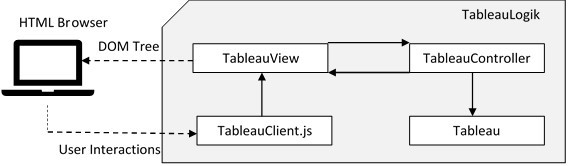
\includegraphics[width=1.0\textwidth]{Achitectur}
\caption[Achitektur]{Achitektur}\label{fig:Achitectur}
\end{figure}
Abbildung \ref{fig:Achitectur} zeigt die Architektur von der Tableau-Webanwendung im Überblick. Die Architektur folgt dem bewährten Model-View-Controller-Prinzip. Softwaretechnisch gliedert sich die
Anwendungslogik so in mehrere Komponenten (Klassen) mit spezifischen funktionalen Verantwortlichkeiten.
%Eine zentrale Rolle für die Anwendungssteuerung hat der Controller (Klasse TableauController). Der Controller kann Nutzerinteraktionen 
%erkennen und in entsprechende Modelinteraktionen umsetzen. Der Controller wird detailliert im Unterabschnitt \ref{subsec:Controller} erläutert.
Die \textit{``TableauClient.js''}
%, die im Unterabschnitt blablabla erläutert
 kann Nutzerinteraktionen erkennen und über den View an den Controller weiterleiten. Der Controller unter entsprechenden Nutzerinteraktionen in 
%Modelinteraktionen 
Model
umsetzen. Der Controller wird detailliert im Unterabschnitt \ref{subsec:Controller} erläutert.

Die \textit{TableauView} kapselt den DOM-Tree und bietet entsprechende Manipulationsmethoden für den Controller an, um sich verändernde Anwendungszustände im Browser zur Anzeige zu bringen. Der View wird im Unterabschnitt \ref{subsec:View} erläutert.

Konzeptionell wird die Tableau-Webanwendung in einem Model abgebildet. Das Model ist komplexer und gliedert sich in mehrere logische Entities, die sich aus den Grundlagen des Kapitels \ref{sec:Grundlagen} ableiten und im Unterabschnitt \ref{sec:Model} erläutert werden.

\section{Klassendiagramm}
Um einen genaueren Überblick zu erhalten, welche Klassen wie mit einander kommunizieren, eignet sich ein Klassendiagramm. Nachfolgend ist zu erkennen, in welcher Kommunikation die Klassen zueinander stehen.
\begin{figure}[ !h] \centering
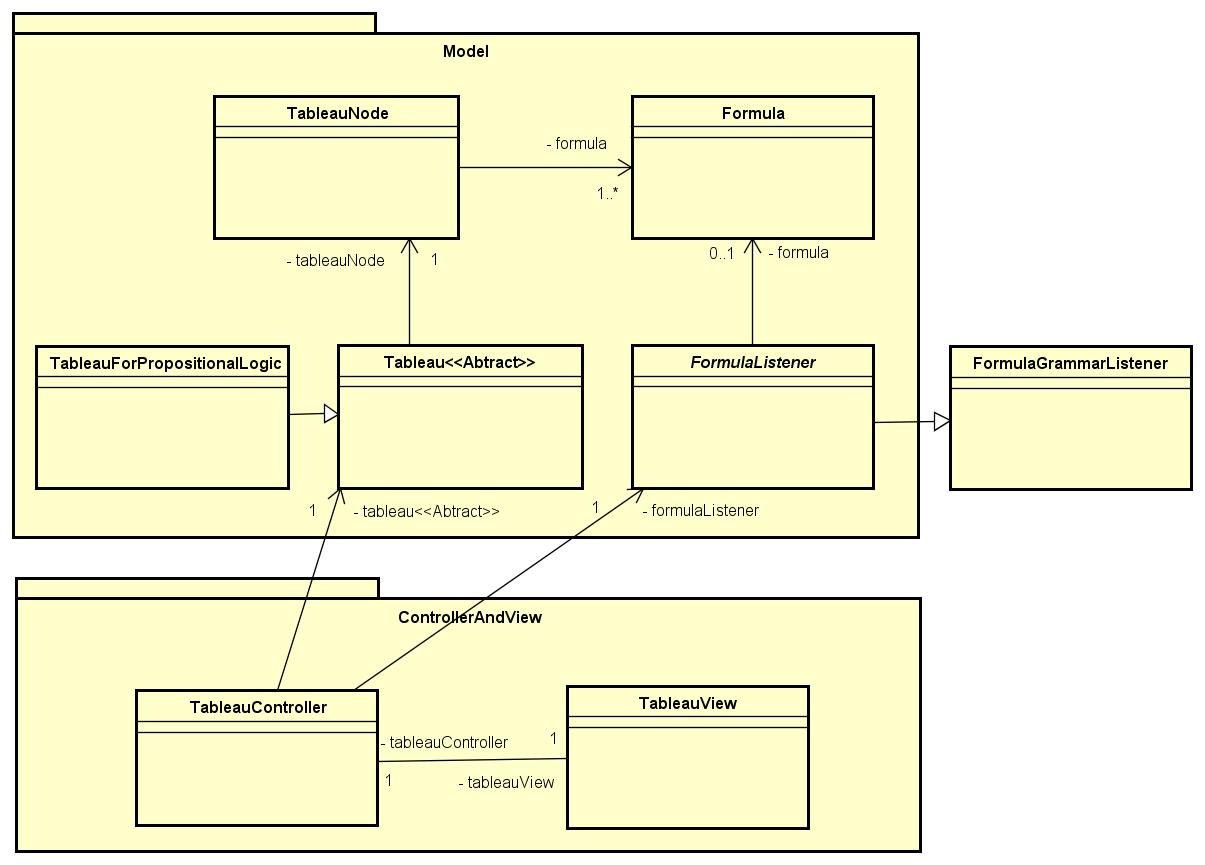
\includegraphics[width=1.0\textwidth]{ClassDiagram}
\caption[Klassendiagramm]{Klassendiagramm}\label{fig:Klassendiagramm}
\end{figure}

Tableau-Webanwendung umfasst verschiedene Bereiche:
\begin{itemize}
\item	Analyse der Eingabeformel und Darstellung einer Formel als Baumstruktur(\hyperlink{/LF10/}{/LF10/}): Klassen \textit{FormulaListener} und \textit{Formula}.
\item	Erstellung und Darstellung des Tableaus (\hyperlink{/LF20/}{/LF20/} und \hyperlink{/LF30/}{/LF30/}):  Klassen \textit{TableauNode}, \textit{Tableau} und \textit{TableauForPropositionalLogic}.
\item	Verarbeitung der GUI-Interaktionen (\hyperlink{/LF10/}{/LF10/}, \hyperlink{/LF20/}{/LF20/}, \hyperlink{/LF30/}{/LF30/} und \hyperlink{/LF40/}{/LF40/}): Klassen \textit{TableauView} und \textit{TableauController}.
\end{itemize}

Um die Möglichkeit zur Erweiterung der Software, gibt es eine abtrakte Klasse \textit{Tableau}, welche die Tableaus erweitern. Die abstrakte Klasse definiert die Basismethoden um ein Tableau zu erstellen. 

